\documentclass{beamer}
\usepackage{mathtools}
\usepackage{amssymb}
\usepackage{amsthm}
\usepackage{physics}
\usepackage{stmaryrd}
\usepackage{bbm}
\usepackage{graphicx}
\usepackage{adjustbox}
\usepackage{hyperref}
\usepackage{tikz}
\usetikzlibrary{angles, quotes}
\usetikzlibrary{calc}
\usepackage{pgfplots}
\usepackage{minted}
\usepackage{subcaption}
\usepackage{algorithm}
\usepackage{algpseudocode}
\usepackage{graphicx}
\usepackage{parskip}
\usepackage{mdframed}
\hypersetup{
    colorlinks=true,
    linkcolor=blue,
    }
\usepackage{biblatex}
\addbibresource{refs.bib}
\useoutertheme{miniframes}

\title{Représentations textuelles et plongements sémantiques : une application pour l'analyse de sentiment}
\author{MARIE Clément, SAMAHA Elio, XIA Tianxiang \\Encadré par Mr. Olivier Schwander}
\date{\today}

\begin{document}
\setbeamertemplate{footline}{%
  \begin{beamercolorbox}[wd=\paperwidth,ht=-1.5ex,dp=1ex]{author in head/foot}%
    \usebeamerfont{author in head/foot}\hfill%
    \insertframenumber\,/\,\inserttotalframenumber\hspace*{2ex}%
  \end{beamercolorbox}%
}
\setbeamertemplate{navigation symbols}{}

\frame{\titlepage}
\begin{frame}
\frametitle{Introduction - Motivation}

\begin{tikzpicture}[remember picture,overlay]
  \node[anchor=north east,inner sep=0pt] at (current page.north east) {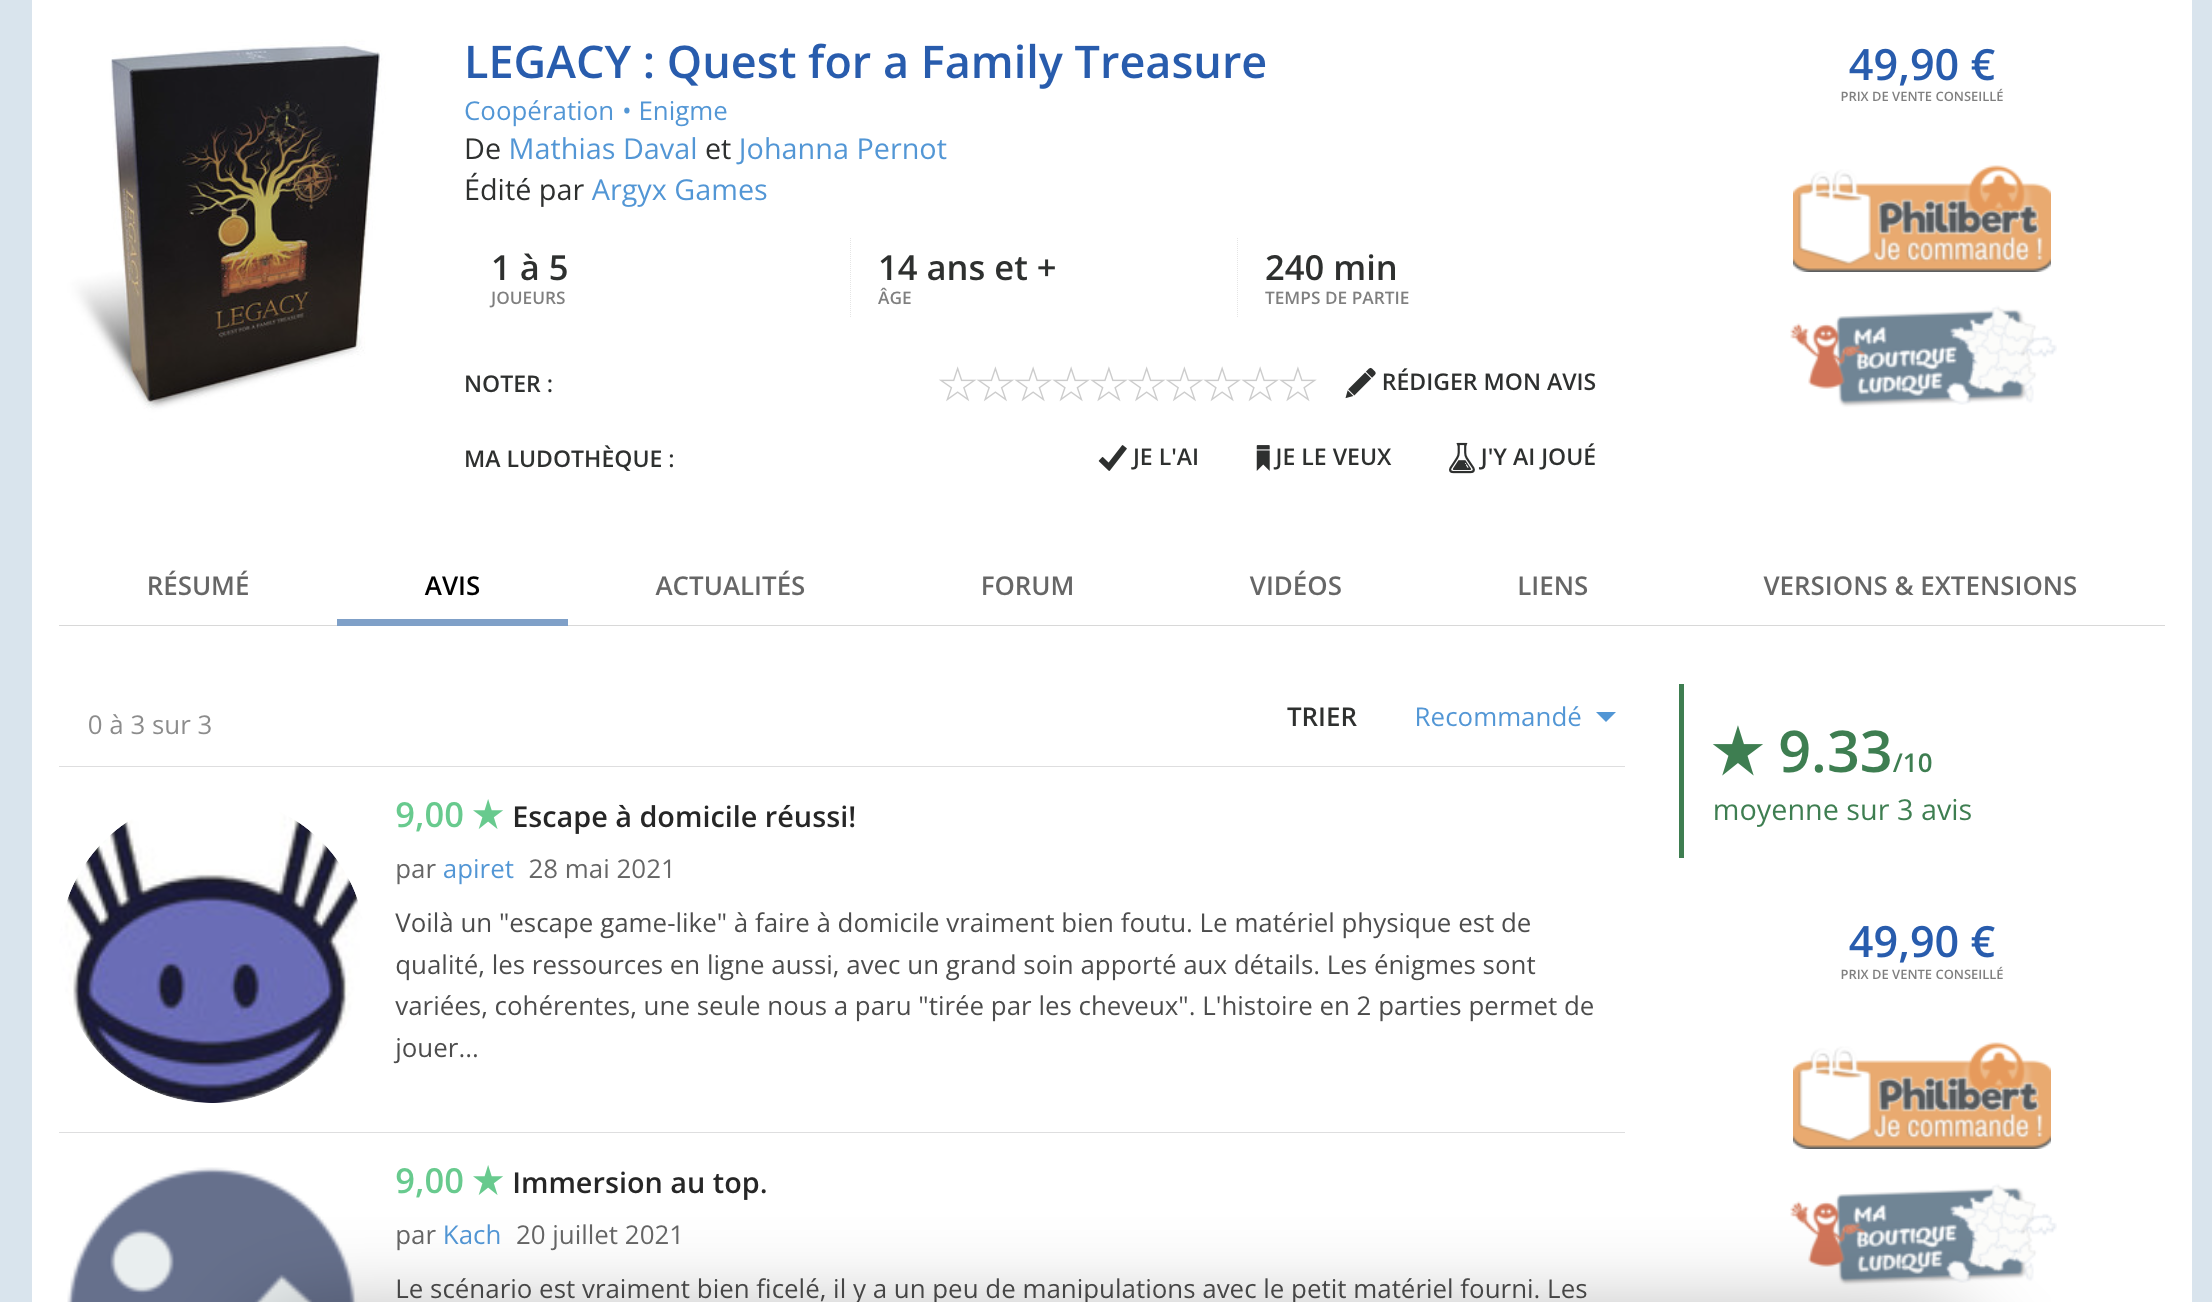
\includegraphics[width=7cm]{tric_trac_pic.png}};
\end{tikzpicture}

\vspace{2.5cm}

\begin{itemize}
  \item Site web Tric Trac: site communautaire autour des jeux de société
  \item Collecte d'avis et de notes des utilisateurs sur les jeux
  \item Traitement de données par représentation vectorielle de mots: analyse multidimensionnelle 
  \item Applications d'algorithmes de classification et évaluation des performances
  \item Enjeux pour l'entreprise   
\end{itemize}
\end{frame}

\begin{frame}
\frametitle{Analyse descriptive des notes: anticipation du problème}

\centering
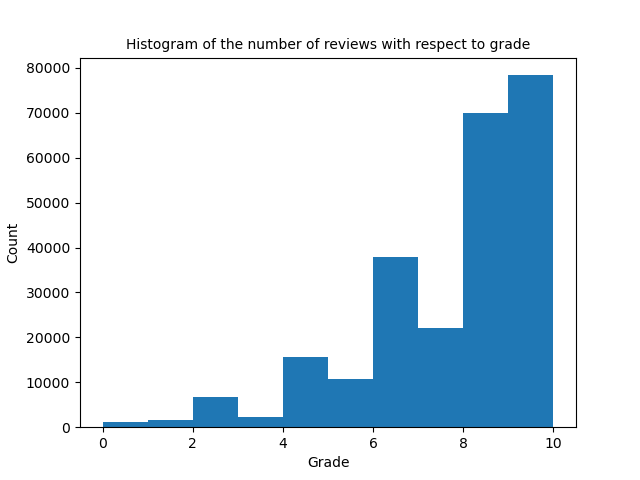
\includegraphics[width=0.8\textwidth]{hist_plot_count.png}

\begin{itemize}
  \item Tendance positive des notes: déséquilibre de classes
  \item Objectif: harmoniser la répresentation positive/négative
  \item Adapter en conséquence les métriques d'évaluation 
\end{itemize}
\end{frame}

\begin{frame}
\frametitle{Représentation vectorielle des documents}
\begin{itemize}
    \item Besoin d'une répresentation numérique: structurée et quantifiable 
    \item Prétraitement (ponctuation, Stemming, stopwords, etc.)
\end{itemize}

\begin{figure}
    \begin{minipage}[b]{0.40\textwidth}
        \centering
        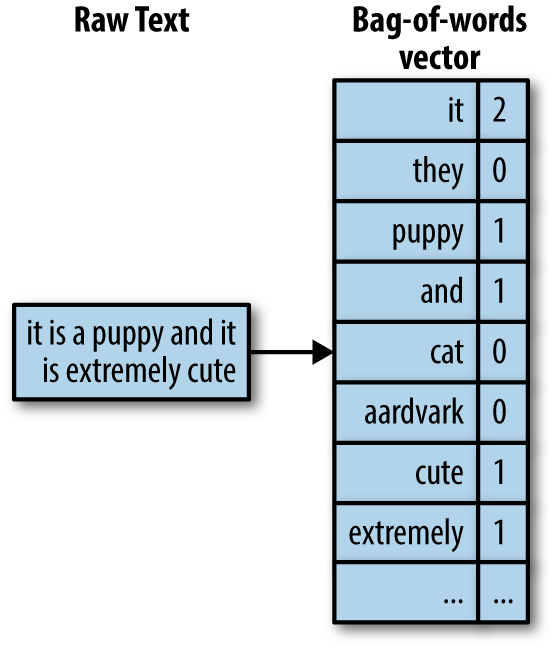
\includegraphics[width=\textwidth]{bag_words.jpeg} 
        \caption{Bag of words}
    \end{minipage}
    \hfill
    \begin{minipage}[b]{0.45\textwidth}
        \centering
        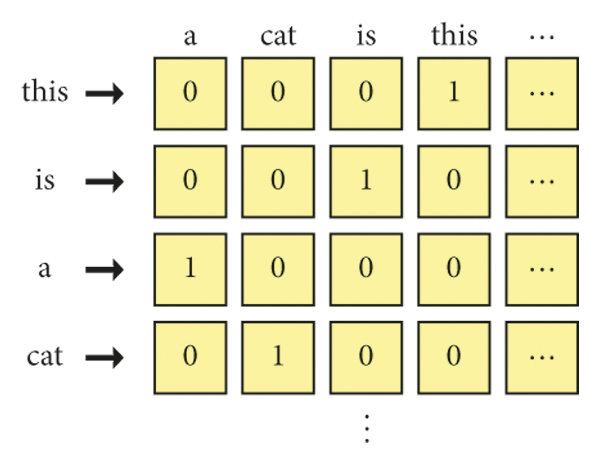
\includegraphics[width=\textwidth]{ohe.png}
        \caption{One Hot Encoding}
    \end{minipage}
\end{figure}
\end{frame}

\begin{frame}
\frametitle{Représentation vectorielle des documents}
\begin{tikzpicture}[overlay, remember picture]
\node[align=center, font=\large\bfseries] at ([yshift=-1.2cm]current page.north) {TF-IDF};
\end{tikzpicture}

formule + explication
\end{frame}

\begin{frame}
\frametitle{Naive Bayes}
\begin{itemize}
    \item CountVectorizer: décompte des occurrences de mots dans le corpus
    \item Algorithme de classification probabiliste
    \item Naif car suppose que les variables sont indépendantes
    \item Probabilités conditionnelles par classe
    \item Classification où la classe prédite maximise la probabilité
\end{itemize}

\begin{figure}
    \begin{minipage}[b]{0.60\textwidth}
        \centering
        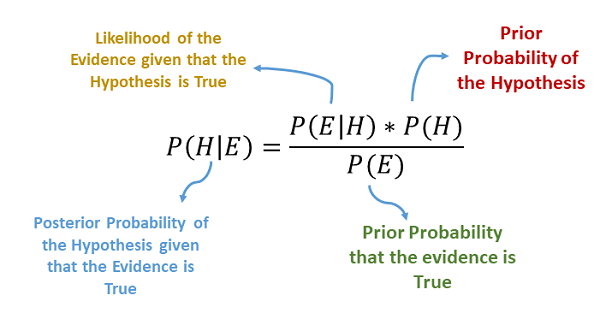
\includegraphics[width=\textwidth]{nb.png} 
        \caption{Théorème de Bayes}
    \end{minipage}
\end{figure}
        
\end{frame}

\begin{frame}
\frametitle{k-nearest neighbors}
\end{frame}

\begin{frame}
\frametitle{Metrics}
\begin{tikzpicture}[overlay, remember picture]
\node[align=center, font=\large\bfseries] at ([yshift=-1.2cm]current page.north) {Naive Bayes};
\end{tikzpicture}

\vspace{1em} % Adjust the vertical spacing between the title and the figures

\caption{Matrices de confusion et métriques associées}
\begin{figure}
    \begin{columns}[T]
    \begin{column}{0.5\textwidth}
        \centering
        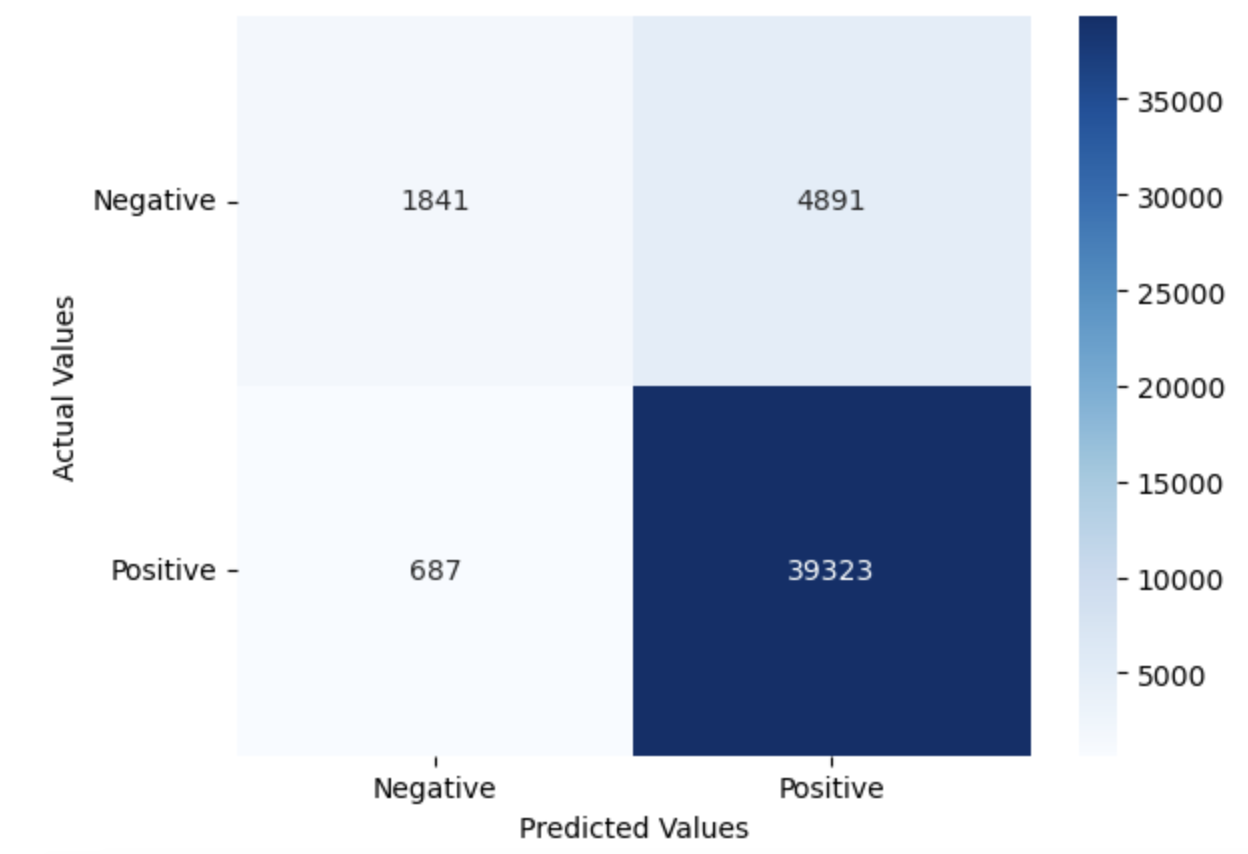
\includegraphics[width=\textwidth]{nb_mat_no_undersampling.png} 
        \caption{Pas d'undersampling}
    \end{column}
    \hfill
    \begin{column}{0.5\textwidth}
        \centering
        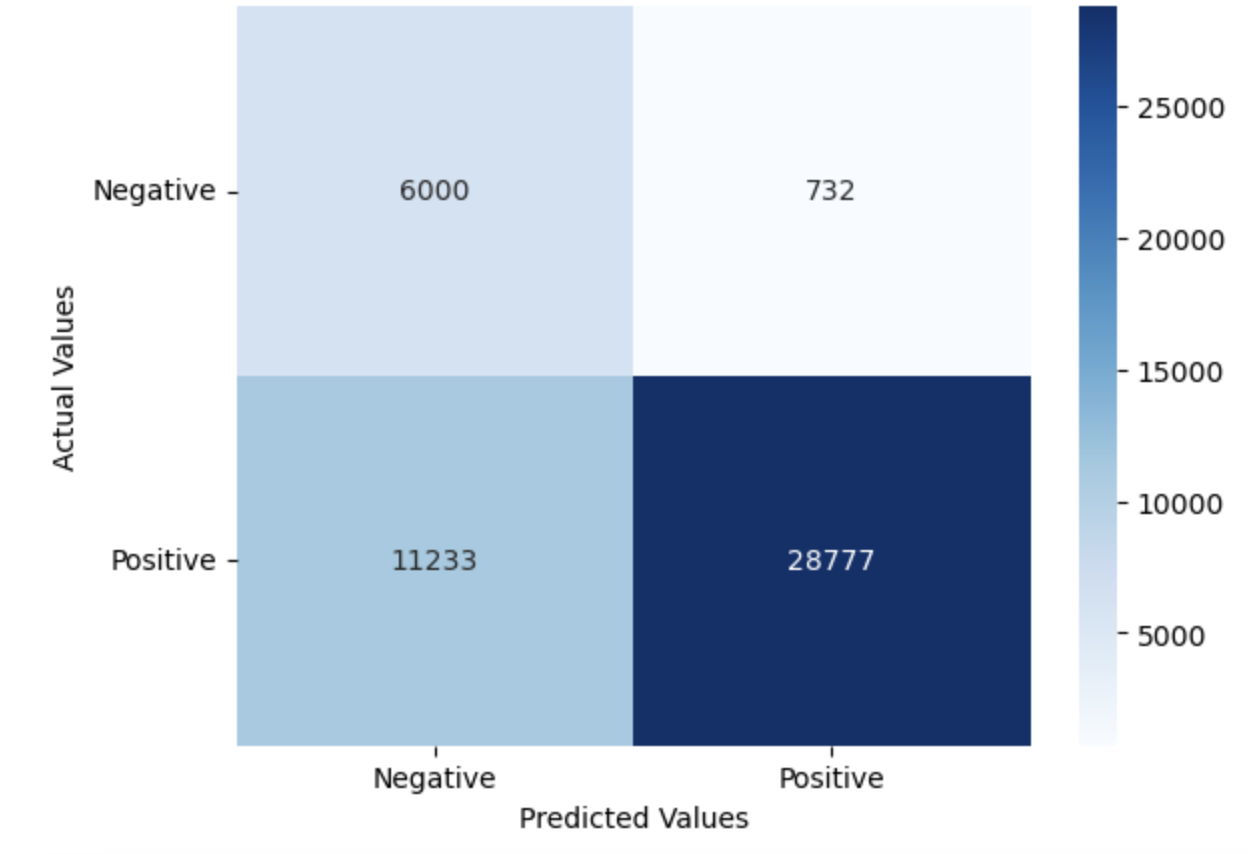
\includegraphics[width=\textwidth]{nb_mat_undersampling.png}
        \caption{Undersampling}
    \end{column}
    \end{columns}
\end{figure}

\begin{table}
\centering
\resizebox{0.6\textwidth}{!}{
\begin{tabular}{cccc}
  & F1 Pos. & F1 Neg. & Accuracy \\
  \hline
  Undersampling & 0.83 & 0.50 & 0.74 \\
  No undersampling & 0.93 & 0.40 & 0.88 \\
\end{tabular}
}
\caption{Metrics}
\label{subfig:scores}
\end{table}
\end{frame}

\begin{frame}
\frametitle{Metrics}
\begin{tikzpicture}[overlay, remember picture]
\node[align=center, font=\large\bfseries] at ([yshift=-1.2cm]current page.north) {k-NN};
\end{tikzpicture}
\end{frame}

\begin{frame}
\frametitle{Persistent homology}
\end{frame}



\end{document}
